% #############################################################################
% This is Chapter 6
% !TEX root = ../main.tex
% #############################################################################
% Change the Name of the Chapter i the following line
\fancychapter{Experimental Work \& Results}
\cleardoublepage
% The following line allows to ref this chapter
\label{chap:results}

So far we have introduced the theme to be developed in this thesis \ref{chap:intro}, we have presented some studies developed in this area \ref{chap:background}, we have presented the concrete case studied in this thesis and we propose a schematization of the work to be developed \ref{chap:architecture}, we have introduced the models that we will implement \ref{chap:Model}, and we have described in detail both the datasets used, as well as the experimental process implemented in this study \ref{chap:implementation}. In this chapter, we present the results obtained in this thesis as well as a discussion section.


\section{Model selection} \label{chap5:framework}

In this section, the process of training and validation of the proposed system begins. In a first stage, the eight architectures of level 1 are trained and validated in order to perform hyperparameter optimization. It is at this stage that the performance of each architecture is evaluated for the training and validation scenario, by performing the block cross-validation procedure. At the end of this stage, the three best models of the eight initially proposed are chosen, and are retrained on the entire dataset 4, used for the block cross-validation, and are tested in a new unseen set of data, dataset 5.

In the second stage, the resulting forecasts of the three models in dataset 5, are used as input for a new model that should compute new forecasts for 5, 10 and 15 minutes. The second phase then consists in developing the level 2 model, trained and validated in dataset 5, where the tuning of its hyperparameters takes place. The total system implemented to test and choose the models, both of level 1 and level 2, is represented in Appendix C, Figure \ref{levels}.

In the third stage, the final results are presented and a comparative analysis is made between the new hybrid ensemble model, and the other simple models.

\subsection{Stage 1 - Level 1 model selection}\label{sec:part1}

The level 1 model selection process, concerns the selection of the three best models, which consists of optimizing the hypterparameters of the eight proposed architectures for level 1, and selecting the best three. To do that, the datasets 1, 2 and 3 represented in Figure \ref{hyptun}, were used, each one consisting of a total of 4 weeks of data, 3 of which were used for training and 1 for validation. The Block cross-validation process described before, is put into practice with these three sets of data, where the eight models are tested and validated in each of the three sets and the errors presented in each of the validation processes are recorded. At the end of this process, an average of the errors presented in each of the three datasets is computed, for the eight architectures, and those presenting the least error are selected. 

\begin{figure}[h!]
    \centering
    \begin{center}
    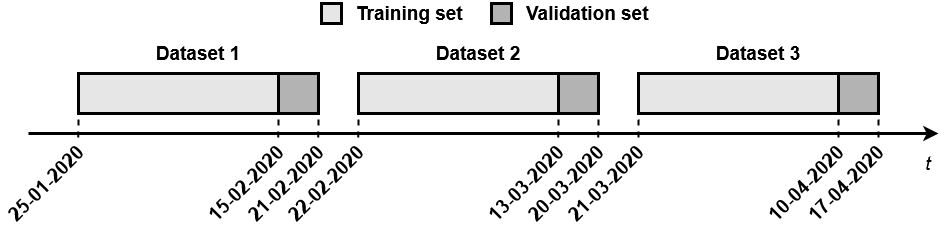
\includegraphics[width=1\textwidth]{Images/hyptun_1.png}
    \caption{Datasets used for training and validation.}
    \label{hyptun}
    \end{center}
\end{figure}

Since the process of tuning the hyperparameters is done by hand, all the architectures started this phase with layers of 8 units. In models 2 and 3 the initial number of filters of the \ac{1D CNN} layers was also 8 and the kernel\_size used was 10. If the models behaved well in the validation set and showed no signs of overfitting or underfitting, the initial values would be maintained. If any of these behaviors were observed in at least one of the datasets, the hyperparameters would be changed, or new layers would be added, until the model presented the desired behavior for all the datasets. It was chosen to start with simple architectures and one would only increase the complexity of the architecture (increasing the number of units per layer, for example) if the model did not present all the desired behavior. The increase in the complexity of the model is associated with an increase in its running time, so it was essential to use models as simple as possible. 


Model 0 consists of a input layer with 15 inputs, a \ac{GRU} layer, and a dense layer for the output with 3 units, one for each forecast ((t+5), (t+10) and (t+15)). In \ac{GRU} layers, the hyperparameter that can be changed is the number of Units - A positive integer that represents the dimensionality of the output space. This hyperparameter must be tuned in to find a value for which the system performs well. However, the increase of this value represents an increase in the complexity of the model, which makes it slower.  In this sense, one tested initially a \ac{GRU} layer with 8 units, for which a good performance was verified.

Regarding Model 1, the structure is relatively similar to Model 0 with the difference that it has an \ac{LSTM} layer instead. Because it typically has a better capacity, this type of layer has more tendency to overfitt, which was verified after some experiments. It was then decided to add a dropout layer with $p$=0.2 to the \ac{LSTM} layer output in order to regularize this situation. This layer has the same number of input and output units, 8.

As before, the number of units defined for the \ac{GRU} and for the \ac{LSTM} layers was 8. Regarding the \ac{1D CNN} layer, some experiments dictated that a good number of filters - An integer that represents dimensionality of the output space (i.e. the number of output filters in the convolution),  to be used could be 8, that is, 8 convolutions are performed that produce the 8 outputs of this layer. The kernel\_size - An integer or tuple/list of a single integer, specifying the length of the 1D convolution window used, was 10 units, which means that the output of this layer consists of the result of consecutive convolutions of 10 values. In the Max pooling layer, a pool\_size of 10 units was also used, which means that only the highest value every 10 values is taken into account, as explained in the section \ref{sec:1dcnn}.

In models 4, 5, 6 and 7, since they have multiple \ac{GRU} and/or \ac{LSTM} layers, the same parameter can be tuned for each one of the layers. These four models represent all possible combinations of two layers composed of \ac{GRU}s and \ac{LSTM}s. In order to avoid overfitting, dopout layers with $p$=0.2 were also added after each of the \ac{GRU} and \ac{LSTM} layers.

In table \ref{tableModels}, a summary of the final models used in the training and validation process can be found. Factors such as the proposed structure and the number of parameters used are detailed.

\begin{table}[htbp]
  \centering
  \caption{Model specifications.}
    \begin{tabular}{r|cccccccc}
    \toprule
    \multicolumn{1}{c|}{\textbf{Model}} & 0     & 1     & 2     & 3     & 4     & 5     & 6     & 7 \\
    \midrule
    \# inputs & 15    & 15    & 15    & 15    & 15    & 15    & 15    & 15 \\
    \# hidden layers & 1     & 2     & 3     & 4     & 4     & 4     & 4     & 4 \\
    \# hidden nodes & 8     & 16    & 24    & 32    & 32    & 32    & 32    & 32 \\
    \# outputs & 3     & 3     & 3     & 3     & 3     & 3     & 3     & 3 \\
    \midrule
    \multicolumn{1}{c|}{\textbf{Model}} & \multicolumn{2}{c}{0} & \multicolumn{2}{c}{1} & \multicolumn{2}{c}{2} & \multicolumn{2}{c}{3} \\
    \midrule
    Layout & \multicolumn{2}{c}{Input (15)} & \multicolumn{2}{c}{Input (15)} & \multicolumn{2}{c}{Input (15)} & \multicolumn{2}{c}{Input (15)} \\
          & \multicolumn{2}{c}{GRU (8)} & \multicolumn{2}{c}{LSTM (8)} & \multicolumn{2}{c}{Conv1D (8, 10)} & \multicolumn{2}{c}{Conv1D (8,10)} \\
          & \multicolumn{2}{c}{Dense (3)} & \multicolumn{2}{c}{Dropout (0.2)} & \multicolumn{2}{c}{Maxpooling(10)} & \multicolumn{2}{c}{Maxpooling(10)} \\
          & \multicolumn{2}{c}{} & \multicolumn{2}{c}{Dense (3)} & \multicolumn{2}{c}{GRU (8)} & \multicolumn{2}{c}{LSTM (8)} \\
          & \multicolumn{2}{c}{} & \multicolumn{2}{c}{} & \multicolumn{2}{c}{Dense (3)} & \multicolumn{2}{c}{Dropout (0.2)} \\
          & \multicolumn{2}{c}{} & \multicolumn{2}{c}{} & \multicolumn{2}{c}{} & \multicolumn{2}{c}{Dense (3)} \\
    \midrule
    \multicolumn{1}{c|}{\textbf{Model}} & \multicolumn{2}{c}{4} & \multicolumn{2}{c}{5} & \multicolumn{2}{c}{6} & \multicolumn{2}{c}{7} \\
    \midrule
    Layout & \multicolumn{2}{c}{Input (15)} & \multicolumn{2}{c}{Input (15)} & \multicolumn{2}{c}{Input (15)} & \multicolumn{2}{c}{Input (15)} \\
          & \multicolumn{2}{c}{GRU (8)} & \multicolumn{2}{c}{LSTM (8)} & \multicolumn{2}{c}{GRU (8)} & \multicolumn{2}{c}{LSTM (8)} \\
          & \multicolumn{2}{c}{Dropout (0.2)} & \multicolumn{2}{c}{Dropout (0.2)} & \multicolumn{2}{c}{Dropout (0.2)} & \multicolumn{2}{c}{Dropout (0.2)} \\
          & \multicolumn{2}{c}{GRU (8)} & \multicolumn{2}{c}{LSTM (8)} & \multicolumn{2}{c}{LSTM (8)} & \multicolumn{2}{c}{GRU (8)} \\
          & \multicolumn{2}{c}{Dropout (0.2)} & \multicolumn{2}{c}{Dropout (0.2)} & \multicolumn{2}{c}{Dropout (0.2)} & \multicolumn{2}{c}{Dropout (0.2)} \\
          & \multicolumn{2}{c}{Dense (3)} & \multicolumn{2}{c}{Dense (3)} & \multicolumn{2}{c}{Dense (3)} & \multicolumn{2}{c}{Dense (3)} \\
    \end{tabular}%
  \label{tableModels}%
\end{table}%

After defining the structural details of the models to be evaluated, a block cross-validation process was then carried out where Datasets 1, 2 and 3 were trained and validated with a distribution of 75\% training and 25\% validation, i.e. three weeks training and one week of validation. In Appendix D, Tables \ref{table4}, \ref{table5} and \ref{table6}, the reader can find the results of the errors presented in each of the three datastes. As it is characteristic of the \ac{RMSE} and the \ac{MAE}, these two error metrics are calculated in original units, that is, the computed errors for the available power are given in Watts, which facilitates the interpretation of the tables.

 In Table \ref{valres} the results of the block cross-validation process can be found, which consists of an average of the errors presented in the three datasets. 


\begin{table}[htbp]
  \centering
  \caption{Stage 1 - Block cross-validation results.}
    \begin{tabular}{cr|cccccccc}
    \toprule
    \multicolumn{1}{l}{\textbf{Model}} &       & 0     & 1     & 2     & \textbf{3} & 4     & 5     & 6     & 7 \\
    \midrule
    \multicolumn{2}{l|}{\textbf{Training Score (t+5)}} &       &       &       &       &       &       &       &  \\
          & RMSE (E+03) & 29.49 & 27.62 & \textbf{26.24} & \textbf{26.43} & 28.00 & 30.12 & 29.23 & \textbf{27.55} \\
          & MAE (E+03) & 22.25 & \textbf{20.42} & \textbf{19.84} & \textbf{19.62} & 20.65 & 22.34 & 21.57 & 20.46 \\
    \multicolumn{2}{l|}{\textbf{Training Score (t+10)}} &       &       &       &       &       &       &       &  \\
          & RMSE (E+03) & 34.13 & 32.81 & \textbf{32.13} & \textbf{32.05} & 32.92 & 34.19 & 34.17 & \textbf{32.31} \\
          & MAE (E+03) & 25.65 & 24.28 & \textbf{24.11} & \textbf{23.77} & 24.34 & 25.32 & 25.30 & \textbf{23.97} \\
    \multicolumn{2}{l|}{\textbf{Training Score (t+15)}} &       &       &       &       &       &       &       &  \\
          & RMSE (E+03) & 37.26 & \textbf{36.19} & 36.23 & \textbf{36.13} & 36.38 & 37.45 & 37.31 & \textbf{35.69} \\
          & MAE (E+03) & 27.93 & \textbf{26.80} & 27.20 & 26.95 & \textbf{26.94} & 27.81 & 27.61 & \textbf{26.48} \\
    \midrule
    \multicolumn{2}{l|}{\textbf{Validation Score (t+5)}} &       &       &       &       &       &       &       &  \\
          & RMSE (E+03) & 39.97 & 33.59 & \textbf{29.11} & \textbf{26.96} & \textbf{30.86} & 35.05 & 39.21 & 35.99 \\
          & MAE (E+03) & 30.06 & 25.58 & \textbf{21.14} & \textbf{20.58} & \textbf{23.97} & 26.77 & 28.96 & 27.90 \\
    \multicolumn{2}{l|}{\textbf{Validation Score (t+10)}} &       &       &       &       &       &       &       &  \\
          & RMSE (E+03) & 46.67 & 35.62 & \textbf{35.59} & \textbf{32.21} & \textbf{34.64} & 37.93 & 41.82 & 39.05 \\
          & MAE (E+03) & 34.80 & 27.59 & \textbf{26.38} & \textbf{24.69} & \textbf{26.92} & 28.89 & 31.54 & 30.26 \\
    \multicolumn{2}{l|}{\textbf{Validation Score (t+15)}} &       &       &       &       &       &       &       &  \\
          & RMSE (E+03) & 48.04 & \textbf{37.87} & 38.11 & \textbf{36.45} & \textbf{37.30} & 41.10 & 43.03 & 41.59 \\
          & MAE (E+03) & 36.29 & 29.35 & \textbf{28.68} & \textbf{28.08} & \textbf{28.81} & 31.47 & 32.40 & 32.13 \\
    \end{tabular}%
  \label{valres}%
\end{table}%


The Table presents the \ac{RMSE} and \ac{MAE} values for each of the eight models, both for training data and validation data, in the forecast for power available in 5, 10 and 15 minutes. It turns out that of all the models tested, the one with the lowest \ac{RMSE} also presents the lowest ac{MAE}, Model 3.Since a more detailed comparative study is intended, the three models with the best validation performance, Models 2, 3 and 4, were chosen. These are the three models with the best performance during Phase 1 for the validation data. It should be noted that for the validation data of (t+15), the \ac{RMSE} value of Model 2 is not among the three best, but Model 1. On the other hand, it can be seen that the \ac{RMSE} value of Model 2 for this situation is quite close to the three best, and since it was the only situation where the value did not present one of the three best performances, this specific case was not taken into account when choosing the three finalist models.



\subsection{Stage 2 - Level 2 model selection}

In the second stage, the goal is to develop, based on the forecasting results obtained by the three level 1 selected models, a model (level 2 model) that combines the results of the three models to generate a single forecasting result (one for each of the three options (t+5), (t+10) and (t+15)). In order to choose the best model to do that, two steps were necessary.

\subsubsection{Input data generation}

In the first step, the three level 1 models selected were retrained, but this time using all the data from datasets 1, 2 and 3, which corresponds to dataset 4, defined in Figure \ref{partition}. The trained models, were then used to predict the power available in the building from 17 April 2020 until 29 May of the same year, corresponding to the dataset 5 defined in Figure \ref{partition}. The results of this procedure can be examined in Table Appendix D, Table \ref{level21}(XXXXXXX MUDAR). The data obtained from the forecasting for each one of the three models is then used as input of level 2. In Figure \ref{level22}, a diagram can be seen that portrays the distribution of information for each dataset across the two levels mentioned.

\begin{figure}[h!]
    \centering
    \begin{center}
    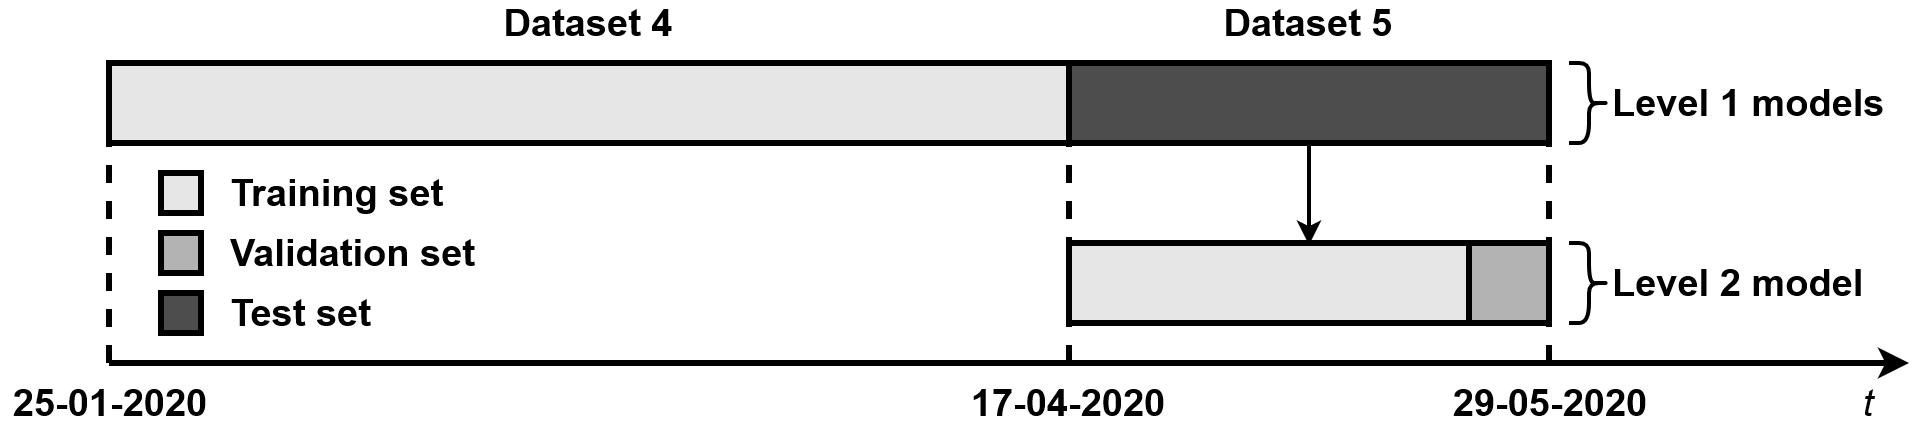
\includegraphics[width=1\textwidth]{Images/stage2.png}
    \caption{Dataset used for testing.}
    \label{level22}
    \end{center}
\end{figure}

The forecasts of (t+5), (t+10) and (t+15) of models 1, 2 and 3 of the first level are used as input for the second level model and as targets, this model has the measured values for the same instant to which the forecasts refer to ((t+5), (t+10) and (t+15)). Table \ref{table:Enseble} details the features used in this process.

\begin{table}[htbp]
  \centering
  \caption{Level 2 model features.}
    \begin{tabular}{rlcl}
    \toprule
          & \multicolumn{1}{c}{\textbf{Feature}} & \textbf{Unit} & \multicolumn{1}{c}{\textbf{Description}} \\
    \midrule
    Input & Model1\_(t+ 5) & W     & Available power prediction of Model 1 for 5 minutes ahead \\
          & Model1\_(t+ 10) & W     & Available power prediction of Model 1 for 10 minutes ahead \\
          & Model1\_(t+ 15) & W     & Available power prediction of Model 1 for 15 minutes ahead \\
          & Model2\_(t+ 5) & W     & Available power prediction of Model 2 for 5 minutes ahead \\
          & Model2\_(t+ 10) & W     & Available power prediction of Model 2 for 10 minutes ahead \\
          & Model2\_(t+ 15) & W     & Available power prediction of Model 2 for 15 minutes ahead \\
          & Model3\_(t+ 5) & W     & Available power prediction of Model 3 for 5 minutes ahead \\
          & Model3\_(t+ 10) & W     & Available power prediction of Model 3 for 10 minutes ahead \\
          & Model3\_(t+ 15) & W     & Available power prediction of Model 3 for 15 minutes ahead \\
    \midrule
    Output & Real (t+5) & W     & Real available power for 5 minutes ahead \\
          & Real (t+10) & W     & Real available power for 10 minutes ahead \\
          & Real (t+15) & W     & Real available power for 15 minutes ahead \\
    \end{tabular}%
  \label{table:Enseble}%
\end{table}%

As input variables, forecasts of each of the selected models of level 1 were chosen. As output variables, the same variables as those present in level 1, Available Power in 5, 10 and 15 minutes, were used. Thus, it is necessary to create a model that can, based on the forecasts obtained for the instants (t+5), (t+10) and (t+15), generate new forecast results for the same instants, using information mutually generated by the three models. Using more information, it is expected that the results are even better.

\subsubsection{Model specifications}


In this second step, it is expected to create a model that, based on the data obtained for the instant (t+5), can obtain new data for (t+5), on the data obtained for the instant (t+10), can obtain new data for (t+10), and based on the data obtained for the instant (t+15), can obtain new data for (t+15). This means that it is no longer necessary to use a \ac{ANN} that can identify temporal patterns, but one that can simply establish a relationship between the input and output data, i.e. it is necessary to apply a \ac{FFNN}. 

As explained in section \ref{chap4:anns}, the best way to do this is to create a \ac{ANN} composed only by layers of the Dense type. In Table \ref{tab:level2arch}, a summary of the specifications of the four evaluated layouts for the level 2 model can be found.

\begin{table}[htbp]
  \centering
  \caption{Level 2 model specifications.}
    \begin{tabular}{c|cccc}
    \toprule
    \textbf{Model} & \multicolumn{4}{c}{Level 2 Model} \\
    \midrule
    Layout & 0     & 1      & 2     & 3 \\
    \midrule
          & Input (12) & Input (12) & Input (12) & Input (12) \\
          & Dense (8) & Dense (16) & Dense (32) & Dense (64) \\
          & Dense (8) & Dense (16) & Dense (32) & Dense (64) \\
          & Dense (3) & Dense (3) & Dense (3) & Dense (3) \\
    \midrule
    \# inputs & 12    & 12    & 12    & 12 \\
    \# hidden layers & 2     & 2     & 2     & 2 \\
    \# hidden nodes & 16    & 32    & 64    & 128 \\
    \# outputs & 3     & 3     & 3     & 3 \\
    \end{tabular}%
  \label{tab:level2arch}%
\end{table}%



For all four layouts, two hidden layers were used. The only hyperparameter that changed from layout to layout was the number of neurons (the size of the output space) in each of the layers, and the combinations of layers of 8 neurons each, two layers of 16 neurons each, two layers of 32 neurons each, and two layers of 64 neurons each were tested. After defining the structural details of level 2 model layouts to be evaluated, a standard validation process was carried out where data from the predictions made by the three level 1 models (which correspond to the time interval of dataset 5), were divided into training and validation with a distribution of 75\% - 25\%, respectively which represents approximately five weeks of data for testing and one week for validation. Table XXX shows the test and validation results for dataset 5, where the four layouts were trained and validated.









\subsection{Stage 3 - Results}

\begin{figure}[h!]
    \centering
    \begin{center}
    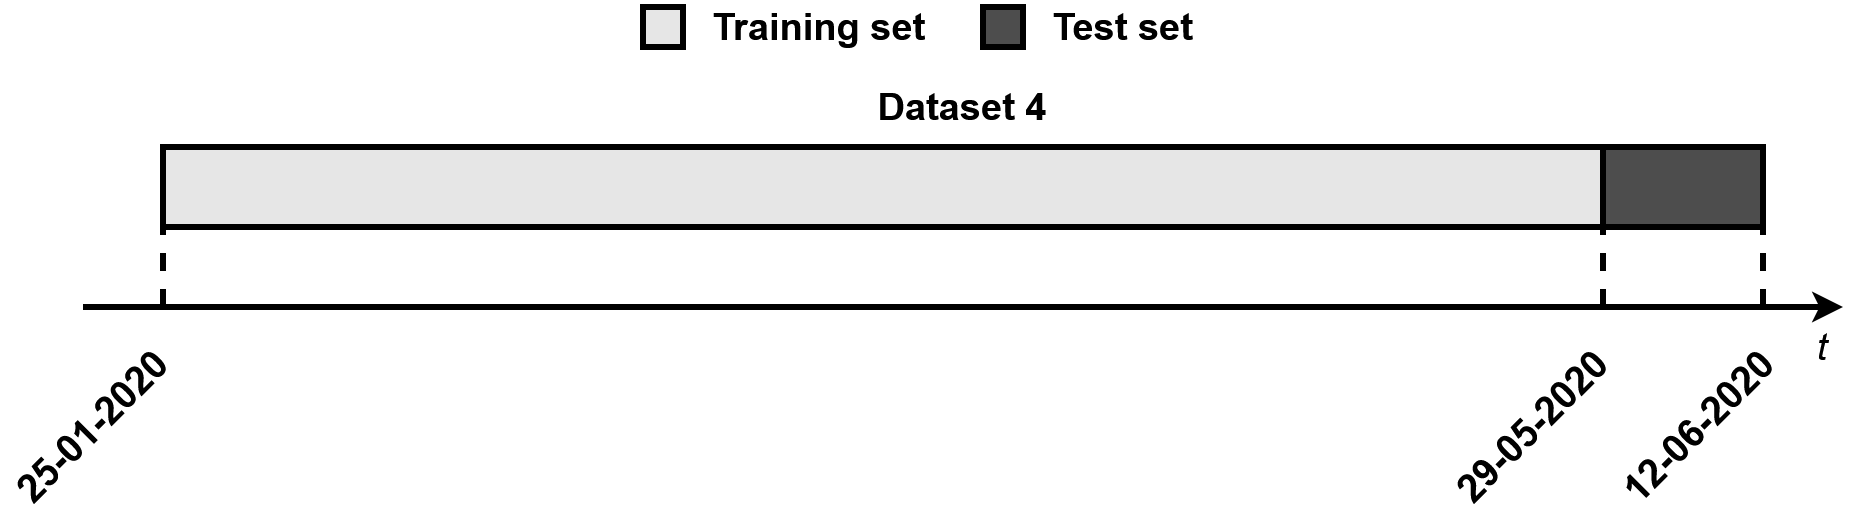
\includegraphics[width=1\textwidth]{Images/Test.png}
    \caption{Dataset used for testing.}
    \label{test}
    \end{center}
\end{figure}

\section{Discussion}


